\documentclass{beamer}				% frames
%\documentclass[notes]{beamer}		% frames + notes
%\documentclass[notes=only]{beamer}	% notes
\documentclass[norsk,a4paper,12pt]{article}
\usepackage[utf8]{inputenc}
\usepackage[english]{babel}
\usepackage{csquotes}	% Supports babel
\usepackage{fancyhdr}
\usepackage{graphicx} %for å inkludere grafikk
\usepackage{verbatim} %for å inkludere filer med tegn LaTeX ikke liker
\usepackage{tabularx}
\usepackage{booktabs}
\usepackage{amsmath}
\usepackage{float}
\usepackage{color}
\usepackage{xcolor}
\usepackage{listings}
\usepackage{hyperref}
\usepackage{amsmath}
\usepackage{tikz}
\usepackage{physics}	% Dirac notation
\usepackage{amssymb}
\usepackage{titlesec}
\usepackage{comment}
\usepackage{fancybox}	% Oval equation box
\usepackage{enumitem}	% Itemize settings
\usepackage{subfig}		% Sub figures
\usepackage{subfloat}	% Figures side by side
\usepackage{geometry}	% Change margins on each page
\usepackage{empheq}		% Beautiful boxes
\usepackage{multirow}	% Multirow in table
\usepackage{multicol}	% Multicolumn in table
\usepackage{varwidth}	% Rotate text in table
\usepackage{arydshln}   % Dashed lines in table

%biblatex
\usepackage[
backend=bibtex,
style=alphabetic,
sorting=ynt
]{biblatex}
\addbibresource{refs.bib}

%listings
\lstset{language=c++}
\lstset{basicstyle=\small}
\lstset{backgroundcolor=\color{white}}
\lstset{frame=single}
\lstset{stringstyle=\ttfamily}
\lstset{keywordstyle=\color{red}\bfseries}
\lstset{commentstyle=\itshape\color{blue}}
\lstset{showspaces=false}
\lstset{showstringspaces=false}
\lstset{showtabs=false}
\lstset{breaklines}
\lstset{postbreak=\raisebox{0ex}[0ex][0ex]{\ensuremath{\color{red}\hookrightarrow\space}}}

%tikz
\setcounter{secnumdepth}{4}
\usetikzlibrary{through, shapes, calc, shapes, arrows, positioning, arrows.meta, shadows}
\tikzstyle{neuron}=[draw,circle,minimum size=20pt,inner sep=0pt, fill=white]
\tikzstyle{stateTransition}=[thick]
\tikzstyle{learned}=[text=red]

%\newcommand{\blds}[1]{\boldsymbol{{#1}}} % better bold in mathmode (from amsmath)
%\newcommand{\Arf}[1]{\Autoref{#1}}
%\renewcommand\normalfont\huge\bfseries\scshape\color{ForestGreen}

%specific reused text
\newcommand{\mdate}{\today}
\newcommand{\mtitle}{Solving Many-body Quantum Problem using Machine Learning}
\newcommand{\mauthor}{Even Marius Nordhagen}
\newcommand{\massignn}{.}

\newcommand{\prtl}{\mathrm{\partial}} %reduce length of partial (less to write)
% \NewDocumentCommand{\prd}{m O{} O{}}{\frac{\prtl^{#3}{#2}}{\prtl{#1}^{#3}}}
\newcommand{\prdp}[2]{\left(\frac{\prtl}{\prtl #1}\right)^{#2}}
\newcommand{\vsp}{\vspace{0.15cm}} %small vertical space
\newcommand{\txtit}[1]{\textit{{#1}}} %italic text
\newcommand{\blds}[1]{\boldsymbol{{#1}}} % better bold in mathmode (from amsmath)
\newcommand{\bigO}{\mathcal{O}} %nice big O
\newcommand{\me}{\mathrm{e}} %straight e for exp
\newcommand{\md}{\mathrm{d}} %straight d for differential
\newcommand{\mRe}[1]{\mathrm{Re}\left({#1}\right)}%nice real
\newcommand{\munit}[1]{\;\ensuremath{\, \mathrm{#1}}} %straight units in math
\newcommand{\Rarr}{\Rightarrow} %reduce lenght of Rightarrow (less to write)
\newcommand{\rarr}{\rightarrow} %reduce lenght of rightarrow (less to write)
\newcommand{\ecp}[1]{\left< {#1} \right>} %expected value
\newcommand{\urw}{\uparrow} % up arrow
\newcommand{\drw}{\downarrow} % down arrow
\newcommand{\pt}[1]{\textbf{\txtit{#1}}\justify}
\newcommand{\infint}{\int\limits^{\infty}_{-\infty}}
\newcommand{\oinfint}{\int\limits^{\infty}_0}
\newcommand{\sint}{\int\limits^{2\pi}_0\int\limits^{\pi}_0\oinfint}
\newcommand{\arcsinh}[1]{\text{arcsinh}\left(#1\right)}
\newcommand{\I}{\scalebox{1.2}{$\mathds{1}$}}
\newcommand{\veps}{\varepsilon} %\varepsilon is to long :P
\newcommand{\cnj}[1]{{#1}^{*}}
\newcommand{\Arf}[1]{\Autoref{#1}}
\newcommand{\suml}[2]{\sum\limits^{#2}_{#1}}
\newcommand{\sumll}[1]{\sum\limits_{#1}}
\newcommand{\tsup}[1]{\textsuperscript{#1}}
\newcommand{\wtld}[1]{\widetilde{#1}}

\newcommand{\ufij}[3]{#1_{#2\rarr#3}}
\newcommand{\Ham}{\hat{H}}
\newcommand{\mb}[1]{\blds{#1}}
\newcommand{\psiTcnj}{\cnj{\Psi}_T(\mb{R};\mb{\alpha})}
\newcommand{\psiT}{{\Psi}_T(\mb{R};\mb{\alpha})}
\newcommand{\phiT}{{\Phi}_T(\mb{R};\mb{\alpha})}
\newcommand{\dinner}[2]{\bra{#1}#2\ket{#1}}
\newcommand{\pinner}{\dinner{\Psi_T}{}}
\newcommand{\langevin}{\prd{t}[r] = DF(r(t)) + \eta}
\newcommand{\rnew}{r^{\text{new}}}
\newcommand{\rold}{r^{\text{old}}}
\newcommand{\Fnew}{F^{\text{new}}}
\newcommand{\Fold}{F^{\text{old}}}
\newcommand{\FokkerPlanck}{\prd{t}[P] = \sum_i D\prd{x_i}\left(\prd{x_i} - \mb{F_i}\right)P}
\newcommand{\Kin}{\frac{1}{2}\sum_i\nabla^2_i}
\newcommand{\frij}{f(\blds{r}_i, \blds{r}_j)}
\newcommand{\fij}{f_{ij}}
\newcommand{\HO}{V(\blds{R}) - \Kin}
\newcommand{\HI}{\sum\limits_{i<j} \frij}
\newcommand{\EHF}{E\left[\Psi^{\text{HF}}\right]}
\newcommand{\HIinnerAS}[2]{\bra{\psi_{#1}\psi_{#2}}H_I\ket{\psi_{#1}\psi_{#2}} - \bra{\psi_{#1}\psi_{#2}}H_I\ket{\psi_{#2}\psi_{#1}}}

\newcommand{\ijnorm}[2]{\sqrt{\braket{#1}{#1}\braket{#2}{#2}}}
\newcommand{\twoDI}{I_{\text{2D}}}
\newcommand{\sumE}[3]{\suml{#1}{#2+#3} E^{#2#3}_{#1}}

\newcommand\CC{C\nolinebreak[4]\hspace{-0.01em}\raisebox{.3ex}{\relsize{-1.35}{\textbf{++}}}\;}
\newcommand{\pp}[1]{#1\nolinebreak[4]\hspace{-.01em}\raisebox{.25ex}{\relsize{-1.5}{\textbf{++}}}\;}

\newcommand{\psiDW}{\psi^{\text{DW}}}
\newcommand{\psiHO}{\psi^{\text{HO}}}
\newcommand{\hDW}{h^{\text{DW}}}
\newcommand{\VDW}{V^{\text{DW}}}
\newcommand{\VHO}{V^{\text{HO}}}
\newcommand{\UDW}{U^{\text{DW}}}

% Define new column alignment types
\newcolumntype{L}[1]{>{\raggedright\let\newline\\\arraybackslash\hspace{0pt}}m{#1}}
\newcolumntype{R}[1]{>{\raggedleft\let\newline\\\arraybackslash\hspace{0pt}}m{#1}}
\newcolumntype{C}{>{\centering\let\newline\\\arraybackslash\hspace{0pt}}X}

% OWN DEFS
\newcommand{\bs}[1]{\boldsymbol{{#1}}}
\newcommand{\detup}{\det(\hat{D}^{\uparrow})}
\newcommand{\detdn}{\det(\hat{D}^{\downarrow})}
\newcommand{\hatH}{\hat{\text{H}}}
\newcommand{\psin}{\Psi_n(\bs{r})}
\newcommand{\psinc}{\Psi_n^*(\bs{r})}
\newcommand{\VMC}{Variational Monte Carlo}
\newcommand{\hatT}{\hat{T}}
\newcommand{\detD}{|\hat{D}|}
\pagestyle{fancy}

\begin{document}

\frontframe

\note{Welcome to my master presentation! It is nice to see that so many of you could be here today! My name is Even, and I will talk about my last years work. It resulted in a master's thesis titled Studies of quantum dots using machine learning. Since I need to compress one years work into 30 minutes, this presentation will not be very technically. For details, I relegate you to this wonderful thesis. }

\mframe{Outline}{}{
\begin{itemize}
	\setlength\itemsep{1em}
	\item Motivation
	\item Quantum Theory
	\item Machine Learning Theory
	\item Methods
	\item Results
	\item Conclusion
	\item (Code)
\end{itemize}
}

\note{We will start with some motivation. Thereafter, we present the essential theory, first quantum theory and then machine learning theory. Our primary focus will be on the results, as that's the most interesting outcome of our work. }

\titleframe{Motivation}

\mframe{}{}{
	\begin{center}
		{\large Studies of Quantum Dots using \textcolor<2>{red}{Machine Learning}}
	\end{center}
}

\note{First I suggest that we take a closer look at the title of my thesis: Studies of Quantum Dots using Machine Learning. We will decompose this to make it more clear, and start with the last term: machine learning.}

\mframe{Machine Learning}{}{
	\begin{itemize}
		\setlength\itemsep{3em}
		\item<1-> \begin{shadequote}{}
			Machine learning is the science of getting computers to act without being explicitly programmed \supercite{noauthor_machine_nodate}.
		\end{shadequote}
		\item<2-> Image recognition 
		\item<3-> Voice commands
	\end{itemize}	
}

\note{Many of you have probbaly heard of the term Machine Learning. To define it, we will use the definition by Stanford university: "Machine learning is the science of getting computers to act without being explicitly programmed." In other words, we don't need to hard-code everything, the machine learning algorithms are supposed to find out what to do themselves. Machine learning has experienced a booming popularity over the past years. Machine learning algorithms are based on studies of the human brain, and are therefore a branch of artificial intelligence. Neural networks have, for instance, revolutioned the field of image recognition, and they make phones and TVs able to recognize your voice.\bigskip

But this is not related to quantum mechanics, why do we want to use machine learning to solve quantum mechanical problems? Do we use it just because it sounds fancy?}

\mframe{Machine Learning + Quantum Mechanics}{}{
	\begin{itemize}
		\item<1-> Neural networks are eminent function approximators
	\end{itemize}	
	\pause\vspace{0.6cm}
	\begin{figure}
		\centering
		\begin{tikzpicture}

% Neural network
\node[input] (output) {};

\node[input, left=5ex of output] (hidden) {};
\node[input, above=3ex of hidden] (hu) {};
\node[input, below=3ex of hidden] (hl) {};

\node[left=6ex of hidden] (visible) {};
\node[input, above=1ex of visible] (vu) {};
\node[input, below=1ex of visible] (vl) {};

\path[draw] (output) -- (hu);
\path[draw] (output) -- (hidden);
\path[draw] (output) -- (hl);

\path[draw] (vu) -- (hu);
\path[draw] (vu) -- (hidden);
\path[draw] (vu) -- (hl);
\path[draw] (vl) -- (hu);
\path[draw] (vl) -- (hidden);
\path[draw] (vl) -- (hl);

% Wave
\node[right=3ex of output, scale=2] (arrow) {$\Rightarrow$};
\begin{axis}[scale=0.4,
	xshift=10ex, 
	yshift=-8ex, 
	axis line style={draw=none}, 
	ticks=none, 
	xmin=-10,
	xmax=10]
	\addplot[thick, black, samples=100, right=2ex of arrow] plot (\x, { (4*\x*\x - 2) * exp(-0.5 * \x*\x) });
\end{axis}

% Psi
\node[left=3ex of visible, scale=2] (equal) {$=$};
\node[left=3ex of equal, scale=3] {$\Psi$};

\end{tikzpicture}

	\end{figure}
	\begin{itemize}
		\item<3-> Existing methods are reminiscent of machine learning algorithms
	\end{itemize}
}

\note{No, there are some good reasons. Firstly, neural networks have shown impressive power as function approximators. In quantum mechanical calculations, the so-called wave function contains all the information about the system, and is therefore our ultimate goal to find.  By approximating the wave function by a neural network, the network can in principle provide all the desired information. \bigskip
Secondly, some quantum many-body methods, like the variational Monte Carlo method that we will discuss later, are similar to machine learning techniques. 
\bigskip
Even though this is a relatively new idea, there exist recent research with the same approach. In 2017, Carlo and Troyer solved the Ising model using restricted Boltzmann machines. A prior student at this group, Flugsrud, extended the work to small quantum dots, and we will again extend her work to larger quantum dots. Recently, Pfau et. al used more traditional neural networks to study atoms and molecules. }

\mframe{}{}{
	\begin{center}
		{\large Studies of \textcolor<2>{red}{Quantum Dots} using Machine Learning}
	\end{center}
}

\note{So now we have discussed the last term, but we will also consider the system that we have investigated: Quantum dots. }

\mframe{Quantum Dots}{}{
	\begin{itemize}
		\setlength\itemsep{3em}
		\item<1-> \textbf{Technologically:} 
		
		Quantum dots are expected to be the next big thing in display technology \supercite{noauthor_samsung_nodate, manders_8.3:_2015}.
		\item<2-> \textbf{Experimentally:}
		
		Researchers have managed to study two-dimensional quantum dots in the laboratory \supercite{brunner_sharp-line_1994}.
		\item<3-> \textbf{Physically:}
		
		An array of interesting physical phenomena can be observed in quantum dots.
	\end{itemize}
}

\note{{\large \textbf{First: What are quantum dots?}}

Quantum dots are small artificial particles, often called artificial atoms because of their many common features with atoms. For instance, both quantum dots and atoms have discrete energy spectra. 

\vspace{0.5cm}
{\large \textbf{There are many reasons why quantum dots are interesting}}

Technologically, quantum dots are expected to be the next big thing in display technology. They have, for instance, the ability to emit light of specific wave lengths, meaning that the color can be controlled with high precision. Samsung already claim that they use quantum dots in their high-end TVs.}

\note{Experimentally, quantum dots can be investigated in the laboratory. This encourage computational experiments as well, since we can use the results from the laboratory experiments as references. Researchers have managed to study quantum dots squeezes between two plates, making the confinement in z-direction absent. This makes them essentially two-dimensional, which is the reason why we have decided to also focus on two-dimensional systems. 
	
	\vspace{0.5cm}
	Physically: From a physical point of view, the quantum dots are interesting as they are simple systems that can model a long range of phenomena. An example is the Wigner localization.
}

\iffalse
\mframe{Why quantum dots?}{}{
	\begin{itemize}
		\item \textbf{Technologically:} 
		
			Quantum dots are expected to be the next big thing in display technology \supercite{noauthor_samsung_nodate, manders_8.3:_2015}.
		\item \textbf{Experimentally:}
		
			Researchers have managed to study two-dimensional quantum dots in the laboratory \supercite{brunner_sharp-line_1994}.
		\item \textbf{Physically:}
		
			An array of interesting physical phenomena can be observed in quantum dots.
	\end{itemize}
}

\note{As mentioned initially, we have focused on quantum dots throughout this thesis. 
	
	\vspace{0.5cm}
	{\large \textbf{But what are quantum dots?}}
	
	Quantum dots are small artificial particles, often called artificial atoms because of their many common features with atoms. For instance, both quantum dots and atoms have discrete energy spectra. 
	
	\vspace{0.5cm}
	{\large \textbf{Why quantum dots?}}
	
	Technologically: Quantum dots are expected to be the next big thing in display technology. They have, for instance, the ability to emit light of specific wave lengths, meaning that the color can be controlled with high precision. Samsung already claim that they use quantum dots in their high-end TVs.
	
}
\note{Experimentally: Quantum dots can be investigated in laboratory experiments. This encourages computational experiments as well, since we can use the results from the laboratory experiments as 		references. Researchers have managed to study quantum dots squeezes between two plates, making the confinement in z-direction absent. This makes them essentially two-dimensional, which is the reason why we have decided to also focus on two-dimensional systems. 
	
	\vspace{0.5cm}
	Physically: From a physical point of view, the quantum dots are interesting as they are simple systems that can model a long range of phenomena. An example is the Wigner localization. 
	
	We will look at circular quantum dots with electron.
}
\fi
\iffalse

\mframe{Why is it challenging?}{}{
	\begin{itemize}
		\item Many-body problem
		\item Fermi-Dirac statistics
		\item Hard to compute the wave function
	\end{itemize}
}

\note{The many-body problem is encountered when simulating a quantum many-body system. The problem is caused by the correlations between the particles. A many-body system means more than two particles.
	
	\vspace{0.5cm}
	Fermionic systems need to obey Fermi-Dirac statistics. This results in the requirement of an anti-symmetric wave function under exchange of two particle coordinates. 
	
	\vspace{0.5cm}
	The wave function is categorized as nondeterministic polynomial hard to compute, which means that...
}

\mframe{How to overcome the challenges?}{}{
	\begin{itemize}
		\item Hartree-Fock (HF) theory
		\item Variational Monte Carlo (VMC) method
		\item Our approach: VMC with Machine Learning \supercite{carleo_solving_2017, pfau2019abinitio}
	\end{itemize}
}

\note{There are several different ways to overcome the many-body problem. The Hartree-Fock method is a popular approach, which, loosely speaking, attempts to replace the electron-electron interactions with a mean field. 
	
	\vspace{0.5cm}
	Then we have the variational Monte Carlo method, which attempts to solve the Schrödinger equation accurately using Monte Carlo integration. It is called variational because we need to introduce a trial wave function ansatz, which we vary. Our approach is to let machine learning define this ansatz, inspired by \citet{carleo_solving_2017} and \citet{flugsrud_vilde_moe_solving_nodate}. Also \citet{pfau2019abinitio} has done something similar. 
}	
\fi

\titleframe{Quantum Theory}

\note{Now we will give a breif introduction to the essential quantum theory.}

\mframe{The Schrödinger Equation}{}{
	\begin{empheq}[box={\mybluebox[5pt]}]{equation}
	\hat{\mathcal{H}}\Psi=E\Psi
	\end{empheq}
	\pause
	\vspace{0.2cm}
	\begin{center}
		{\large $\Downarrow$}
	\end{center}
	\vspace{0.3cm}
	\begin{equation}
	E=\frac{\int d\bs{X}\Psi^*(\bs{X})\hat{\mathcal{H}}\Psi(\bs{X})}{\int d\bs{X}\Psi^*(\bs{X})\Psi(\bs{X})}
	\end{equation}
}

\note{The Schrödinger equation describes the motion of any quantum mechanical system, and is the equation that I have spent one year solving. Since we will limit us to stationary systems only, the time-independent Schrödinger equation will be our focus. In linear algebra terms, it is an eigenvalue equation with the Hamilton operator, $\hat{\mathcal{H}}$, as a matrix and the wave function, $\Psi$, as the eigen function. $E$ is the energy, which is the eigenvalue.

\vspace{0.5cm}
The most natural way of solving this equation, is to simply express the Hamiltonian as a matrix and obtain the wave function and the energy from diagonalizing the matrix. This is known as configuration interaction. However, we can only do this for small systems, as it is very computational intensive. 
}

\note{Instead, we separate the equation with respect to the energy, and obtain a equation consisting of some integrals. This equation is hard to solve due to the electron-electron correlations. }

\mframe{The Variational Principle}{}{
	
	
	The variational principle serves as a way of finding the ground state energy. For an arbitrary trial wave function $\Psi_T(\bs{X})$, it states that the obtained energy is larger or equal to the ground state,
	\begin{equation}
	E_0\leq E=\frac{\int d\bs{X}\Psi_T^*(\bs{X})\hat{\mathcal{H}}\Psi_T(\bs{X})}{\int d\bs{X}\Psi_T^*(\bs{X})\Psi_T(\bs{X})}.
	\end{equation}
	Thus, by minimizing the obtained energy, $E$, we can estimate the ground state energy. 
}

\note{We also have the variational principle, which is used by variational methods to obtain the ground state energy. Loosely speaking, it states that by solving this integral with an arbitrary wave function, $\Psi_T$, the obtained energy is always larger or equal to the ground state energy. This means that we can estimate the ground state energy by minimizing the obtained energy.}

\titleframe{Machine Learning Theory}

\note{Now over to the machine learning theory.}

\mframe{Feed-forward Neural Network (FNN)}{}{
	\begin{figure}[scale=0.2]
		\centering
		\begin{tikzpicture}

% Define outputs
\node[] (center) {};
\node[input, above=0.3em of center] (y1) {};
\node[input, below=0.3em of center] (y2) {};

% Draw lines from output nodes
\node[right of=y1] (righty1) {};
\node[right of=y2] (righty2) {};
\path[draw,->] (y1) -- (righty1);
\path[draw,->] (y2) -- (righty2);

% Hidden nodes L
\node[input,left=5em of center] (aL3) {};
\node[input,above of=aL3] (aL2) {};
\node[input,above of=aL2] (aL1) {};
\node[input,below of=aL3] (aL4) {};
\node[input,below of=aL4] (aL5) {};

% Hidden nodes 1
\node[input,left=15em of center] (a13) {};
\node[input,above of=a13] (a12) {};
\node[input,above of=a12] (a11) {};
\node[input,below of=a13] (a14) {};
\node[input,below of=a14] (a15) {};

% Draw lines from hidden nodes
\path[draw,->] (aL1) -- (y1);
\path[draw,->] (aL2) -- (y1);
\path[draw,->] (aL3) -- (y1);
\path[draw,->] (aL4) -- (y1);
\path[draw,->] (aL5) -- (y1);

\path[draw,->] (aL1) -- (y2);
\path[draw,->] (aL2) -- (y2);
\path[draw,->] (aL3) -- (y2);
\path[draw,->] (aL4) -- (y2);
\path[draw,->] (aL5) -- (y2);

% Define place left of left
\node[input,left=5em of a13] (x2) {};
\node[input,above of=x2] (x1) {};
\node[input,below of=x2] (x3) {};

% Draw lines from input nodes
\path[draw,->] (x1) -- (a11);
\path[draw,->] (x1) -- (a12);
\path[draw,->] (x1) -- (a13);
\path[draw,->] (x1) -- (a14);
\path[draw,->] (x1) -- (a15);

\path[draw,->] (x2) -- (a11);
\path[draw,->] (x2) -- (a12);
\path[draw,->] (x2) -- (a13);
\path[draw,->] (x2) -- (a14);
\path[draw,->] (x2) -- (a15);

\path[draw,->] (x3) -- (a11);
\path[draw,->] (x3) -- (a12);
\path[draw,->] (x3) -- (a13);
\path[draw,->] (x3) -- (a14);
\path[draw,->] (x3) -- (a15);

% Draw lines from first hidden layer
\path[draw,->] (a11) -- (aL1);
\path[draw,->] (a11) -- (aL2);
\path[draw,->] (a11) -- (aL3);
\path[draw,->] (a11) -- (aL4);
\path[draw,->] (a11) -- (aL5);

\path[draw,->] (a12) -- (aL1);
\path[draw,->] (a12) -- (aL2);
\path[draw,->] (a12) -- (aL3);
\path[draw,->] (a12) -- (aL4);
\path[draw,->] (a12) -- (aL5);

\path[draw,->] (a13) -- (aL1);
\path[draw,->] (a13) -- (aL2);
\path[draw,->] (a13) -- (aL3);
\path[draw,->] (a13) -- (aL4);
\path[draw,->] (a13) -- (aL5);

\path[draw,->] (a14) -- (aL1);
\path[draw,->] (a14) -- (aL2);
\path[draw,->] (a14) -- (aL3);
\path[draw,->] (a14) -- (aL4);
\path[draw,->] (a14) -- (aL5);

\path[draw,->] (a15) -- (aL1);
\path[draw,->] (a15) -- (aL2);
\path[draw,->] (a15) -- (aL3);
\path[draw,->] (a15) -- (aL4);
\path[draw,->] (a15) -- (aL5);


% Draw lines towards input nodes
\node[left of=x1] (leftx1) {};
\node[left of=x2] (leftx2) {};
\node[left of=x3] (leftx3) {};
\path[draw,->] (leftx1) -- (x1);
\path[draw,->] (leftx2) -- (x2);
\path[draw,->] (leftx3) -- (x3); 
\end{tikzpicture}
	\end{figure}
}

\mframe{Restricted Boltzmann machines}{}{
	\begin{figure}[width=5cm]
		\centering
		\begin{tikzpicture}

% Define visible units
\node[input] (x2) {$x_2$};
\node[input] at (1,+3/2) (x1) {$x_1$};
\node[input] at (1,-3/2) (x3) {$x_3$};

% Define hidden units
\node[input] at (3,+3/2) (h1) {$h_1$};
\node[input] at (4,0) (h2) {$h_2$};
\node[input] at (3,-3/2) (h3) {$h_3$};

% Define biases
\node[input] at (0,7/2) (a) {$1$};
\node[input] at (4,7/2) (b) {$1$};

% Define paths
\path[draw,thick,-] (x1) -- (h1) node[midway,above] {$w_{11}$};
\path[draw,thick,-] (x1) -- (h2);
\path[draw,thick,-] (x1) -- (h3);

\path[draw,thick,-] (x2) -- (h1);
\path[draw,thick,-] (x2) -- (h2);
\path[draw,thick,-] (x2) -- (h3);

\path[draw,thick,-] (x3) -- (h1);
\path[draw,thick,-] (x3) -- (h2);
\path[draw,thick,-] (x3) -- (h3);

\draw[color3,thick,-] (b) to [out=270,in=90] (h1);
\draw[color3,thick,-] (b) to [out=315,in=45] (h2);
\draw[color3,thick,-] (b) to [out=0,in=0] (h3) node[] at (6,1) {$b_3$};

\draw[color1,thick,-] (a) to [out=270,in=90] (x1);
\draw[color1,thick,-] (a) to [out=225,in=135] (x2);
\draw[color1,thick,-] (a) to  [out=180,in=180] (x3) node[] at (-2,1) {$a_3$};


% Add some text
\node[below=1em of x3] {visible};
\node[below=1em of h3] {hidden};
\end{tikzpicture}

	\end{figure}
}

\titleframe{Methods}

\note{Similar to the theory, also the methods that we have used will be discussed briefely.}

\mframe{Variational Monte Carlo (VMC)}{}{
	Exploit the variational principle in order to obtain the ground state energy
	\begin{equation}
	\begin{aligned}
	E_0 < E_{\text{VMC}} &= \frac{\int d\bs{R}\Psi_T(\bs{R})^*\hat{\mathcal{H}}\Psi_T(\bs{R})}{\int d\bs{R}\Psi_T(\bs{R})^*\Psi_T(\bs{R})},\\
	%&= \int d\bs{R}\underbrace{\frac{\Psi_T(\bs{R})^*\Psi_T(\bs{R})}{\int d\bs{R}\Psi_T(\bs{R})^*\Psi_T(\bs{R})}}_{P(\bs{R})}\cdot\underbrace{\frac{1}{\Psi_T(\bs{R})}\hat{\mathcal{H}}\Psi_T(\bs{R})}_{E_L(\bs{R})}\\
	&=\int d\bs{R}E_L(\bs{R})P(\bs{R}),
	\end{aligned}
	\end{equation}
	with
	\begin{equation}
	E_L(\bs{R})=\frac{1}{\Psi_T(\bs{R})}\hat{\mathcal{H}}\Psi_T(\bs{R})\quad\wedge\quad P(\bs{R})=\frac{\Psi_T(\bs{R})^*\Psi_T(\bs{R})}{\int d\bs{R}\Psi_T(\bs{R})^*\Psi_T(\bs{R})}
	\end{equation}
}

\note{The variational Monte Carlo method, which our work is based on, exploits the variational principle in order to obtain an estimate of the ground state energy. We also rewrite the integral in terms of the local energy, $E_L$, and the probability density function $P(\bs{R})$. }

\mframe{Monte Carlo Integration}{}{
	We attempt to solve the integral by sampling from the probability density function $P(\bs{R})\propto\Psi_T(\bs{R})^*\Psi_T(\bs{R})$:
	\begin{equation}
	\begin{aligned}
	E_{\text{VMC}} &= \int d\bs{R} E_L(\bs{R})P(\bs{R}),\\
	&\approx\frac{1}{M}\sum_{i=1}^ME_L(\bs{R}_i).
	\end{aligned}
	\end{equation}
}

\note{By doing this, the integral becomes in the form of a general expectation value, which straightforward can be approached using Monte Carlo integration, shown here with $M$ Monte Carlo cycles. This does only give an energy, but by adjusting the trial wave function, $\Psi_T$, in order to minimize the energy and repeat the exercise multiple times, we may estimate the ground state energy. }

\mframe{Trial Wave Function Ansatz}{}{
	
	The Slater-Jastrow function is the \textit{de facto} standard trial wave function for electronic structure systems,
	\begin{equation}
	\Psi_T(\bs{R})=|\hat{D}(\bs{R})|J(\bs{R}),
	\end{equation}
	where the Slater matrix,
	\begin{equation}
	\hat{D}(\bs{R})=
	\begin{pmatrix}
	\phi_1(\boldsymbol{r}_1) & \phi_2(\boldsymbol{r}_1) & \hdots & \phi_N(\boldsymbol{r}_1)\\
	\phi_1(\boldsymbol{r}_2) & \phi_2(\boldsymbol{r}_2) & \hdots & \phi_N(\boldsymbol{r}_2)\\
	\vdots & \vdots & \ddots & \vdots \\
	\phi_1(\boldsymbol{r}_N) & \phi_2(\boldsymbol{r}_N) & \hdots & \phi_N(\boldsymbol{r}_N)
	\end{pmatrix},
	\end{equation}
	contains all the single-particle functions.
}

\note{The trial wave function can in principle be an arbitrary function with a few requirements. For electron systems, like our quantum dots, the wave function has to be anti-symmetric under exchange of two coordinates. The standard trial wave function for this purpose is named the Slater-Jastrow function and consists of a Slater determinant, $|\hat{D}(\bs{R})|$, to introduce the anti-symmetry and a Jastrow factor, $J(\bs{R})$, to model the electron-electron correlations. The function inside the Slater matrix are called the single-particle functions...}

\mframe{Single-particle Functions}{}{
	The Hermite functions,
	\begin{equation}
	\phi_n(\bs{r})\propto H_n(\bs{r})\exp(-\frac{1}{2}\alpha\omega|\bs{r}|^2),
	\end{equation}
	are often used as the single-particle functions for quantum dots. The Gaussian can be factorized out from the Slater determinant,
	\begin{equation}
	|\hat{D}(\bs{R};\alpha)|\propto\exp(-\frac{1}{2}\alpha\omega|\bs{R}|^2)
	\begin{vmatrix}
	H_1(\boldsymbol{r}_1) & H_2(\boldsymbol{r}_1) & \hdots & H_N(\boldsymbol{r}_1)\\
	H_1(\boldsymbol{r}_2) & H_2(\boldsymbol{r}_2) & \hdots & H_N(\boldsymbol{r}_2)\\
	\vdots & \vdots & \ddots & \vdots \\
	H_1(\boldsymbol{r}_N) & H_2(\boldsymbol{r}_N) & \hdots & H_N(\boldsymbol{r}_N)
	\end{vmatrix}.
	\end{equation}
}

\note{...and are traditionally taylored to every particular system. For quantum dots, the Hermite functions are often used as the single-particle functions. Here, $H_n$ is the Hermite polynomial of $n$'th order, $\omega$ is the frequency (strength) of the quantum dot and $\alpha$ is a variational parameter. An important finding, is that the gaussian part (point) can be factorized out from the Slater determinant such that the determinant no longer contains variational parameters. Our contribution is to let a restricted Boltzmann machine control the single-particle function...}

\mframe{Restricted Boltzmann Machine}{}{
	As suggested by \citet{carleo_solving_2017}, we use the marginal distribution of the visible units as the single-particle functions in the Slater determinant, and see if them can model the correlations 
	\begin{equation}
	\phi_n(\bs{r})\propto H_n(\sqrt{\omega}\bs{r})P(\bs{r};\bs{\theta})
	\end{equation}
	where $P(\bs{r})$ is the marginal distribution of the visible units.
	\begin{equation}
	|\hat{D}(\bs{r};\bs{\theta})|\propto P(\bs{r};\bs{\theta})
	\begin{vmatrix}
	H_1(\boldsymbol{r}_1) & H_2(\boldsymbol{r}_1) & \hdots & H_N(\boldsymbol{r}_1)\\
	H_1(\boldsymbol{r}_2) & H_2(\boldsymbol{r}_2) & \hdots & H_N(\boldsymbol{r}_2)\\
	\vdots & \vdots & \ddots & \vdots \\
	H_1(\boldsymbol{r}_N) & H_2(\boldsymbol{r}_N) & \hdots & H_N(\boldsymbol{r}_N)
	\end{vmatrix}
	\end{equation}
}

\note{...as suggested by Carleo and Troyer. We then simply replace the Gaussian part by the marginal distribution of a restricted Boltzmann machine and obtain this expression of the determinant. This serves our goal because we no longer need to taylor the single-particle functions to the system, making it require less physical intuition. }


\mframe{Jastrow Factor}{}{
The Jastrow factor is added to account for the correlations

Simple Jastrow factor
\begin{equation}
J(\bs{r}; \bs{\beta}) = \exp(\sum_{i=1}^N\sum_{j>i}^N{\beta_{ij}r_{ij}}).
\end{equation}

Padé-Jastrow factor
\begin{equation}
J(\bs{r};\beta) = \exp(\sum_{i=1}^N\sum_{j>i}^N\frac{a_{ij}r_{ij}}{1+\beta r_{ij}}).
\end{equation}
}

\note{We also mentioned the Jastrow factor, which can be added in order to model the electron-electron correlations. We have decided to study two different Jastrow factors. The simple Jastrow factor does only contain variational parameters, $\beta_{ij}$, multiplied with the relative distances between the particles, $r_{ij}$, and contains a minimum of physical intuition. It is interesting since we want to develop a method that does not require a significant amount of physical intuition. The Padé-Jastrow factor is, on the other hand, taylored to model the electron-electron correlations correctly, and contains therefore more physical information. $\beta$ is a variational parameter and $a_{ij}$ is a factor depending on the electrons $i$ and $j$. }

\mframe{Our Trial Wave Function Ansätze}{}{
	\begin{itemize}
		\setlength\itemsep{3em}
		\item $\Psi_{\text{RBM}}(\bs{R})=|\hat{D}(\bs{R})|$
		\item $\Psi_{\text{RBM+SJ}}(\bs{R})=|\hat{D}(\bs{R})|J(\bs{R};\bs{\beta})$
		\item $\Psi_{\text{RBM+PJ}}(\bs{R})=|\hat{D}(\bs{R})|J(\bs{R};\beta)$
		\item $\Psi_{\text{VMC}}(\bs{R})=|\hat{D}(\bs{R})|J(\bs{R};\beta)$
	\end{itemize}
}

\note{We end up with four wave function ansätze: We have the RBM ansatz, which is just the Slater determinant with the restricted Boltzmann machines as the single-particle functions. Then we have the RBM+SJ ansatz, which is simply the RBM ansatz multiplied with the simple Jastrow factor. We also have the RBM ansatz multiplied with the Padé-Jastrow factor, denoted by the RBM+PJ ansatz. In the end, we have the standard Slater-Jastrow ansatz also containing the Padé-Jastrow factor which we call the VMC ansatz. In the following, we will compare their performance in the form of results. }

\titleframe{Results}

\mframe{Ground State Energy}{Number of electrons: $N=2$. Frequency: $\omega$.}{
\begin{table}
	%\caption{$N=2$}
	\begin{tabularx}{\textwidth}{lR{1.25cm}R{1.25cm}R{1.4cm}R{1.4cm}R{1.2cm}R{1.cm}} 
		\toprule
		$\omega$ & RBM & RBM+SJ & RBM+PJ & VMC & HF \footnote{Computation of the Hartree-Fock limit by \citeauthor{mariadason_quantum_2018}, \citeyear{mariadason_quantum_2018} \cite{mariadason_quantum_2018}.} & Exact \footnote{Semi-analytical ground state energy calculated by \citeauthor{taut_two_1993}, \citeyear{taut_two_1993} \cite{taut_two_1993}.} \\
		\midrule \\
		1/6 & 0.7036(1) & 0.67684(7) & 0.66715(6) & 0.66710(1) & 0.768675 & 2/3 \\ 
		1 & 3.0803(2) & 3.02108(5) & 2.999587(5) & 2.99936(1) & 3.16190 & 3 \\
		\bottomrule
	\end{tabularx}
\end{table}
}

\note{The first results that I would like to present, is the ground state energy of a couple of quantum dots that we know the exact energy of. More precisely, we look at quantum dots with two electrons and frequency $\omega=1/6$ and 1. We see here that the RBM ansatz, in the first column, provides energies not very far from the analytical energies in this last column. They are also lower than the Hartree-Fock limit, which is interesting as the Hartree-Fock algorithm attempts to find the optimal Slater determinant without Jastrow factors. When we add more intuition in form of the simple Jastrow factor, the energy drops further towards the exact energy. The RBM+PJ ansatz is totally on pair with the VMC ansatz. }

\mframe{Ground State Energy}{Number of electrons: $N=20$. Frequency: $\omega$.}{
\begin{table}
	%\caption{$N=20$}
	\begin{tabularx}{\hsize}{lR{1.25cm}R{1.25cm}R{1.3cm}R{1.4cm}R{1.cm}R{1.4cm}} \\
		\toprule
		$\omega$ & RBM & RBM+SJ & RBM+PJ & VMC & HF \footnote{Computation of the Hartree-Fock limit by \citeauthor{mariadason_quantum_2018}, \citeyear{mariadason_quantum_2018} \cite{mariadason_quantum_2018}.} & DMC \footnote{Ground state energy estimate using the diffusion Monte Carlo method. By \citeauthor{hogberget_quantum_2013}, \citeyear{hogberget_quantum_2013} \cite{hogberget_quantum_2013}.} \\
		\midrule \\
		0.1 & 30.824(2) & 30.567(3) & 30.1553(9) & 30.0403(2) & 31.1902 & 29.9779(1) \\ 
		%0.28 & 63.788(4) & 62.786(3) & 62.148(1) & 63.5390 & 62.0755(7) & 61.9268(1) \\
		%0.5 & 96.410(1) & 94.920(4) & 94.104(1) & 95.7328 & 94.0433(9) & 93.8752(1) \\
		1.0 & 159.428(3) & 156.816(4) & 156.104(1) & 155.8900(4) & 158.004 & 155.8822(1) \\ 
		\bottomrule
	\end{tabularx}
\end{table}
}

\note{We also investigate quantum dots with 20 electrons and frequencies $\omega=0.1$ and 1.0. For these systems, we do not have analytically energy, but we use the diffusion Monte Carlo energy as reference, which is believed to be more or less exact. What we see is that the RBM ansatz again is not far from the reference, but for high frequency the energy is larger than the Hartree-Fock limit. This illustrates that RBM is better at modelling correlations than Hartree-Fock. }

\mframe{Energy distribution}{Number of electrons: $N=20$. Frequency: $\omega$.}{
	Ratio between the kinetic energy, $\langle\hat{T}\rangle$, and the total potential energy, $\langle\hat{V}\rangle$.
	\begin{figure}
		\centering 
		\begin{tikzpicture}

\begin{axis}[
legend cell align={left},
legend style={at={(0.9,0.1)}, anchor=south east, draw=white!80.0!black},
title style={yshift=-1.5ex},
%tick align=outside,
tick pos=both,
x grid style={white!69.01960784313725!black},
xlabel={\(\displaystyle \omega\)},
width=8cm,
height=6cm,
xmajorgrids,
xmin=-0.4895, xmax=10.4995,
xtick style={color=black},
y grid style={white!69.01960784313725!black},
ylabel style={rotate=-90.0},
ylabel={\(\displaystyle \frac{\langle\hat{T}\rangle}{\langle\hat{V}\rangle}\)},
ymajorgrids,
%ymin=-0.03, ymax=0.7,
ytick style={color=black}
]
\addplot [thick, color0]
table {%
	0.01 0.0202855736090596
	0.1 0.0558188176084186
	0.28 0.0748673013733255
	0.5 0.092181964299863
	1 0.120447174205168
	2 0.191577362501107
	3 0.2257693437
	5 0.263982205508037
	10 0.278872126802915
};
\addlegendentry{RBM}
\addplot [thick, color1]
table {%
	0.01 0.0224807471735212
	0.1 0.0510365183964855
	0.28 0.0535270823545204
	0.5 0.0761996706229769
	1 0.108428284656055
	2 0.17366909653192
	3 0.19307880632568
	5 0.260942252768941
	10 0.332349732889548
};
\addlegendentry{RBM+SJ}
\addplot [thick, color2]
table {%
	0.01 0.0198390540318607
	0.1 0.0550696242390316
	0.28 0.0812272164373049
	0.5 0.0960548685344326
	1 0.120346512979882
	2 0.152555093728466
	3 0.20363356015151
	5 0.286590458917023
	10 0.373618884667807
};
\addlegendentry{RBM+PJ}
\addplot [thick, color3]
table {%
	0.01 0.0164511376657391
	0.1 0.0430938843433643
	0.28 0.067074638154502
	0.5 0.0907330085826954
	1 0.121087634122869
	2 0.176534004132603
	3 0.20481414099371
	5 0.307872099467483
	10 0.330233868695407
};
\addlegendentry{VMC}
\end{axis}
\end{tikzpicture}
		%\caption{$N=20$}
	\end{figure}
}

\note{We also look at the distribution between kinetic energy and total potential energy. Keep looking at quatum dots with 20 electrons, we see that the potential energy dominates over the potential energy when the frequency gets low. Also, the various ansätze differ more for high frequencies. }

\mframe{One-body density}{Number of electrons: $N=20$. Frequency: $\omega=1.0$.}{
	\begin{figure}
		\centering
		\captionsetup[subfigure]{labelformat=empty}
		\subfloat{\raisebox{1cm}{\rotatebox[origin=t]{90}{RBM}}}\hspace{0.cm}
		\subfloat{{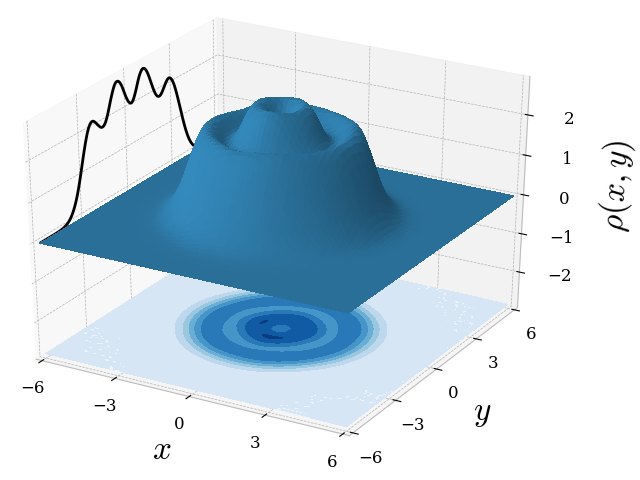
\includegraphics[width=3cm]{../plots/int1/onebody2/2D/20P/1.000000w/RBM_ADAM_MC1048576.png}}}\hspace{0.5cm}
		\subfloat{\raisebox{1cm}{\rotatebox[origin=t]{90}{RBM+SJ}}}\hspace{0.cm}
		\subfloat{{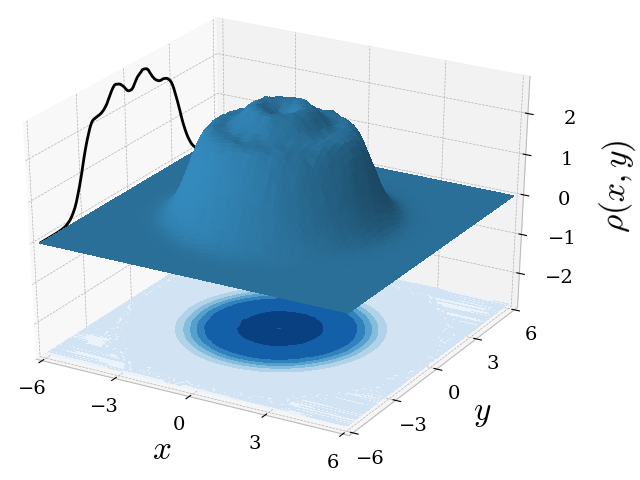
\includegraphics[width=3cm]{../plots/int1/onebody2/2D/20P/1.000000w/RBMSJ_ADAM_MC1048576.png}}}\\
		\subfloat{\raisebox{1cm}{\rotatebox[origin=t]{90}{RBM+PJ}}}\hspace{0.cm}
		\subfloat{{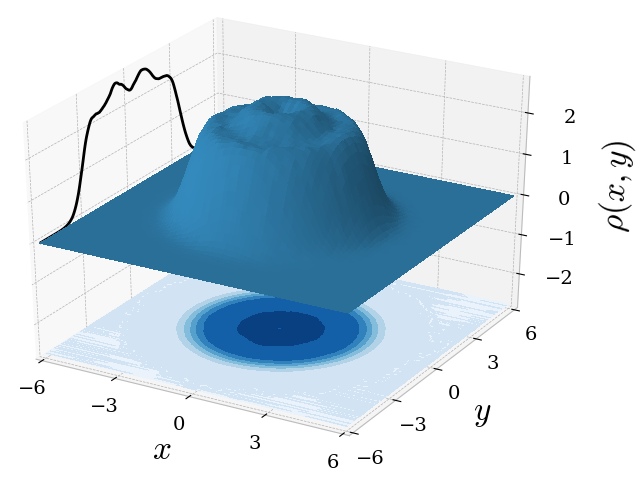
\includegraphics[width=3cm]{../plots/int1/onebody2/2D/20P/1.000000w/RBMPJ_ADAM_MC1048576.png}}}\hspace{0.5cm}
		\subfloat{\raisebox{1cm}{\rotatebox[origin=t]{90}{VMC}}}\hspace{0.cm}
		\subfloat{{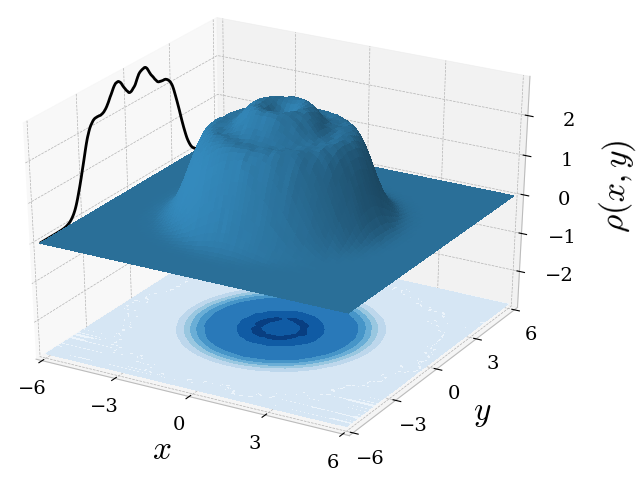
\includegraphics[width=3cm]{../plots/int1/onebody2/2D/20P/1.000000w/VMC_ADAM_MC1048576.png}}}
		%\caption{$N=20$, $\omega=1.0$}
	\end{figure}
}

\note{Now, we look at the one-body density provided by the varius ansätze. We observe that all the ansätze with a Jastrow factor, i.e. RBM+SJ, RBM+PJ and VMC, provide very similar density profiles, while RBM provides more distinct peaks. It looks like the RBM ansatz manages to find the same extrema as the other ansätze, but determines another density there. }

\mframe{Two-body density}{Number of electrons: $N=20$. Frequency: $\omega=1.0$.}{
	\begin{figure}
		\centering
		\captionsetup[subfigure]{labelformat=empty}
		\subfloat{\raisebox{1cm}{\rotatebox[origin=t]{90}{RBM}}}\hspace{0.cm}
		\subfloat{{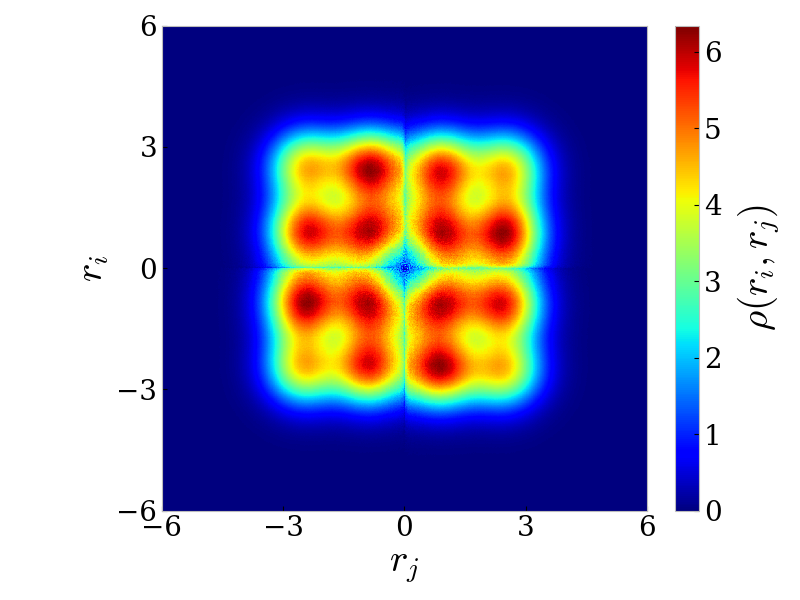
\includegraphics[width=3cm]{../plots/int1/twobody/2D/20P/1.000000w/RBM_ADAM_MC1048576.png}}}\hspace{0.5cm}
		\subfloat{\raisebox{1cm}{\rotatebox[origin=t]{90}{RBM+SJ}}}\hspace{0.cm}
		\subfloat{{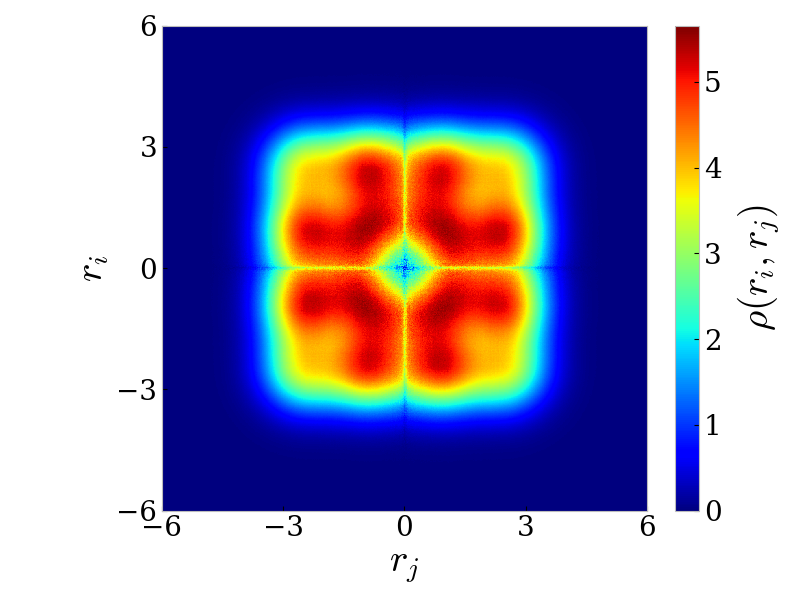
\includegraphics[width=3cm]{../plots/int1/twobody/2D/20P/1.000000w/RBMSJ_ADAM_MC1048576.png}}}\\
		\subfloat{\raisebox{1cm}{\rotatebox[origin=t]{90}{RBM+PJ}}}\hspace{0.cm}
		\subfloat{{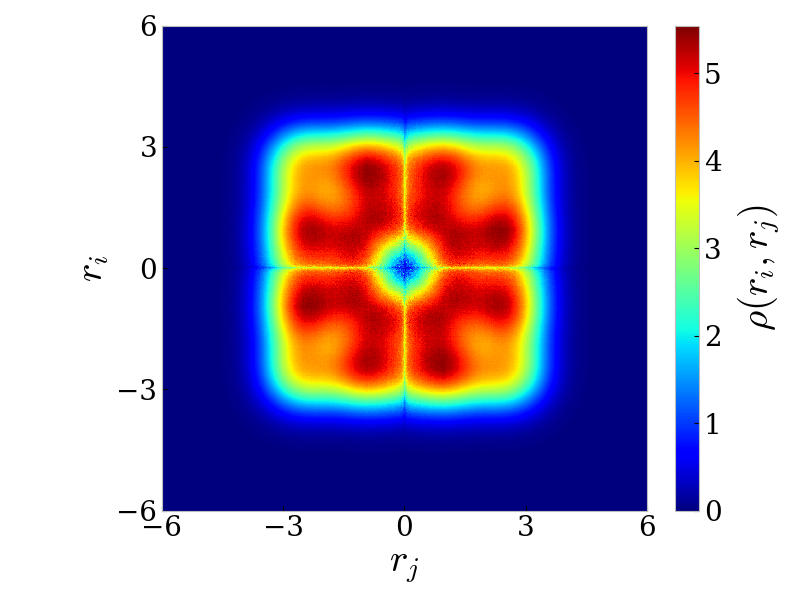
\includegraphics[width=3cm]{../plots/int1/twobody/2D/20P/1.000000w/RBMPJ_ADAM_MC1048576.png}}}\hspace{0.5cm}
		\subfloat{\raisebox{1cm}{\rotatebox[origin=t]{90}{VMC}}}\hspace{0.cm}
		\subfloat{{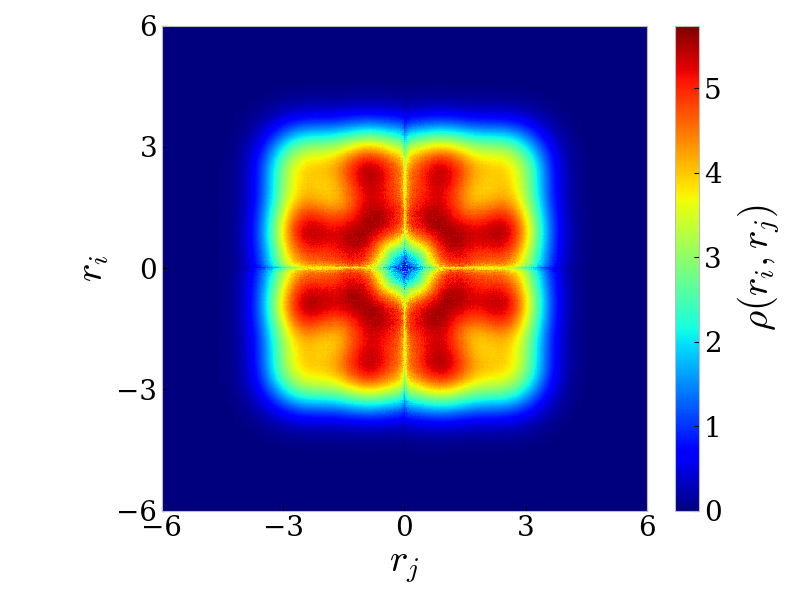
\includegraphics[width=3cm]{../plots/int1/twobody/2D/20P/1.000000w/VMC_ADAM_MC1048576.png}}}
		%\caption{$N=20$, $\omega=1.0$}
	\end{figure}
}

\note{We have also studied the two-body density, which makes us able to study the electron-electron correlations in more detail. A similar phenomenon as we saw for the one-body density can be observed in the two-body density. RBM provides more distinct peaks than its fellow ansätze. }

\mframe{Low-frequency dots}{Number of electrons: $N$. Frequency: $\omega=0.1$.}{
	\begin{figure}
		\centering
		\captionsetup[subfigure]{labelformat=empty}
		\subfloat{\raisebox{1cm}{\rotatebox[origin=t]{90}{RBM}}}\hspace{0.1cm}
		\subfloat{{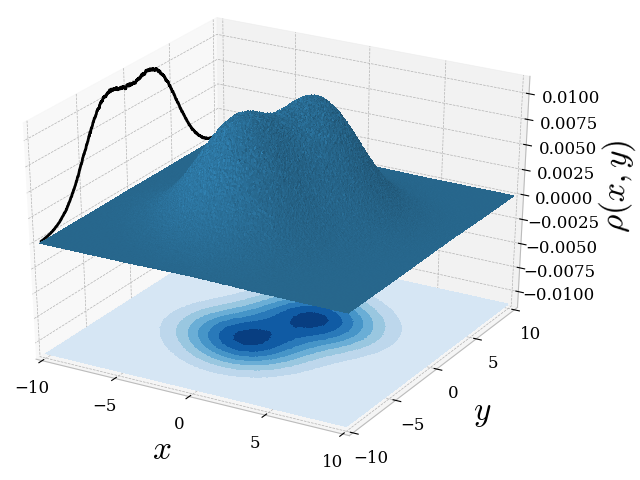
\includegraphics[width=3cm]{../plots/int1/onebody2/2D/2P/0.100000w/RBM_ADAM_MC1048576.png}}}\hspace{-0.cm}
		\subfloat{{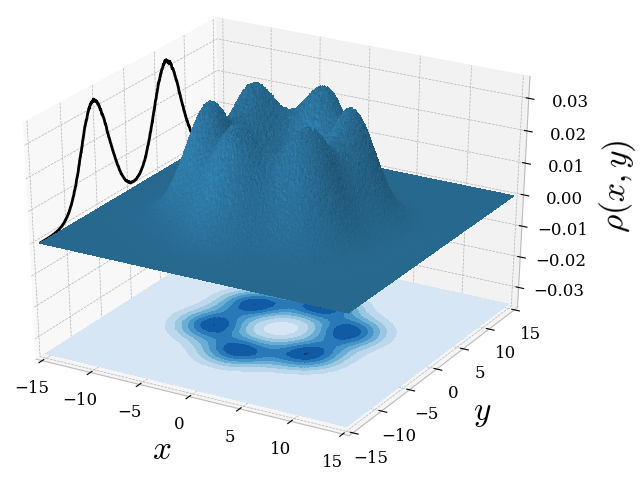
\includegraphics[width=3cm]{../plots/int1/onebody2/2D/6P/0.100000w/RBM_ADAM_MC1048576.png}}}\hspace{-0.cm}
		\subfloat{{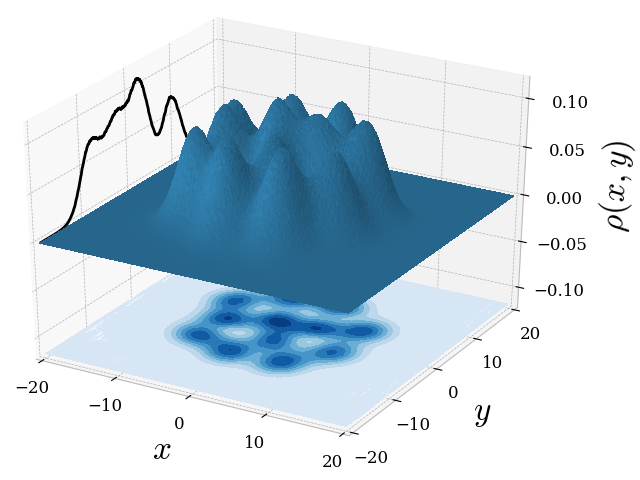
\includegraphics[width=3cm]{../plots/int1/onebody2/2D/12P/0.100000w/RBM_ADAM_MC1048576.png}}}\\ [-0.cm]
		
		\subfloat{\raisebox{1cm}{\rotatebox[origin=t]{90}{VMC}}}\hspace{0.1cm}
		\subfloat[$N=2$]{{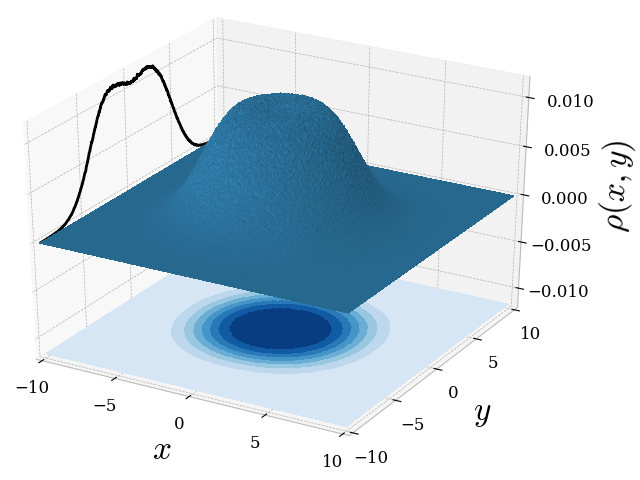
\includegraphics[width=3cm]{../plots/int1/onebody2/2D/2P/0.100000w/VMC_ADAM_MC1048576.png}}}\hspace{-0.cm}
		\subfloat[$N=6$]{{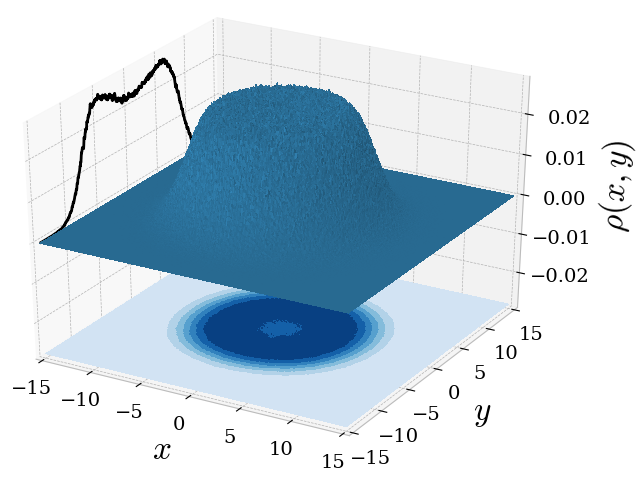
\includegraphics[width=3cm]{../plots/int1/onebody2/2D/6P/0.100000w/VMC_ADAM_MC1048576.png}}}\hspace{-0.cm}
		\subfloat[$N=12$]{{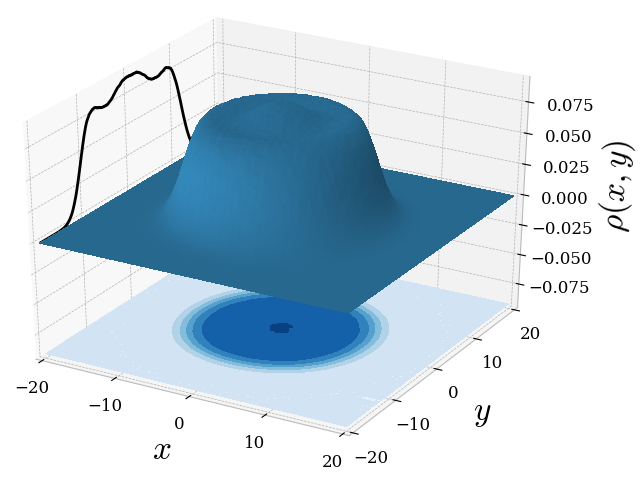
\includegraphics[width=3cm]{../plots/int1/onebody2/2D/12P/0.100000w/VMC_ADAM_MC1048576.png}}}
		%\caption{$\omega=0.1$}
	\end{figure}
}

\note{We now move on to quantum dots with frequency $\omega=0.1$. When comparing the RBM ansatz and the VMC ansatz, we see that the two ansätze give very different one-body density profiles. Apparently, the RBM ansatz provides an equal number of peaks as there are electrons, implying very localized particle positions. What is interesting, is that the energy is the respective methods are quite similar. This indicates that the energy itself might not be the best way to decide whether an ansatz is good or not. }

\mframe{Computational Cost}{Number of electrons: $N$.}{
	\begin{figure}
		\centering 
		% This file was created by matplotlib2tikz v0.7.4.
\begin{tikzpicture}[scale=0.9]

\begin{axis}[name=2D, xlabel=$N$, ylabel={CPU-time [s]}, grid=major, legend pos=north west, xtick=data] 
\addplot[color=color1,mark=oplus*, dashed] coordinates { 
	(2,6.05)
	(6,11.25)
	(12,20.53) 
	(20,38.99) 
	(30,73.73) 
	(42,130.49) 
	(56,213.47)
	(72,360.22)
	(90,856.84) }; 
\addlegendentry{RBM};

\addplot[color=color2,mark=oplus*, dash dot] coordinates { 
	(2,7.12) 
	(6,14.07) 
	(12,28.42) 
	(20,63.27) 
	(30,122.93) 
	(42,199.60)
	(56,349.22)}; 
\addlegendentry{RBM+SJ};

\addplot[color=color3,mark=oplus*, dotted] coordinates { 
	(2,7.26)
	(6,13.50)
	(12,27.68)
	(20,57.09) 
	(30,119.17) 
	(42,212.53) 
	(56,382.13) }; 
\addlegendentry{RBM+PJ};

\addplot[color=color0,mark=oplus*] coordinates { 
	(2,5.11)
	(6,10.51)
	(12,20.85) 
	(20,41.20) 
	(30,76.26) 
	(42,137.39) 
	(56,230.63)
	(72,355.81)
	(90,544.03) }; 
\addlegendentry{VMC};
\end{axis}
\end{tikzpicture}
	\end{figure} 
}

\note{In the end, we will also compare the computational cost of the various methods. From the graphs, we see that the RBM and VMC ansätze are pairwise the computationally cheapest methods and RBM+SJ and RBM+PJ are the most computational intensive ones. This is no big surprise, as the two latter methods contain bith a neural network and a Jastrow factor. We also see that the cost of the RBM ansatz explodes for very large systems. This is probably because the ansatz then contains around 15,000 variational parameters, while the VMC ansatz contains two variational parameters. }

\titleframe{Conclusions}

\note{Now we will address some brief conclusions. }

\mframe{Conclusions}{}{
	\begin{itemize}
		\setlength\itemsep{3em}
		\item RBM is able to account for most of the correlations
		\item RBM+PJ implies to give a lower ground state energy and model the correlations better than a traditional VMC
		\item RBM+SJ is both more expensive and less accurate than its fellow methods, and we see no reason to choose it
	\end{itemize}
}

\mframe{Future Work}{}{
	\begin{itemize}
		\setlength\itemsep{3em}
		\item Repeat the exercise using spherical coordinates - interactions are easier to model in spherical coordinates
		\item Check the ability of modeling the three-body correlations, considering nuclear systems
		\item Reduce the computational cost
	\end{itemize}
}

\titleframe{Thank you!}

\note{Thank you all for listening! Since I have a few more minutes, I will show how the developed software can be used. }

\mframe{References}{}{
	\printbibliography
}

\end{document}